\subsection{بخش د}
در این بخش به بررسی درنظرگرفتن زاویه پیشبین در قانون هدایت فرمان به خط دید پرداخته شده است.
\begin{figure}[H]
	\centering
	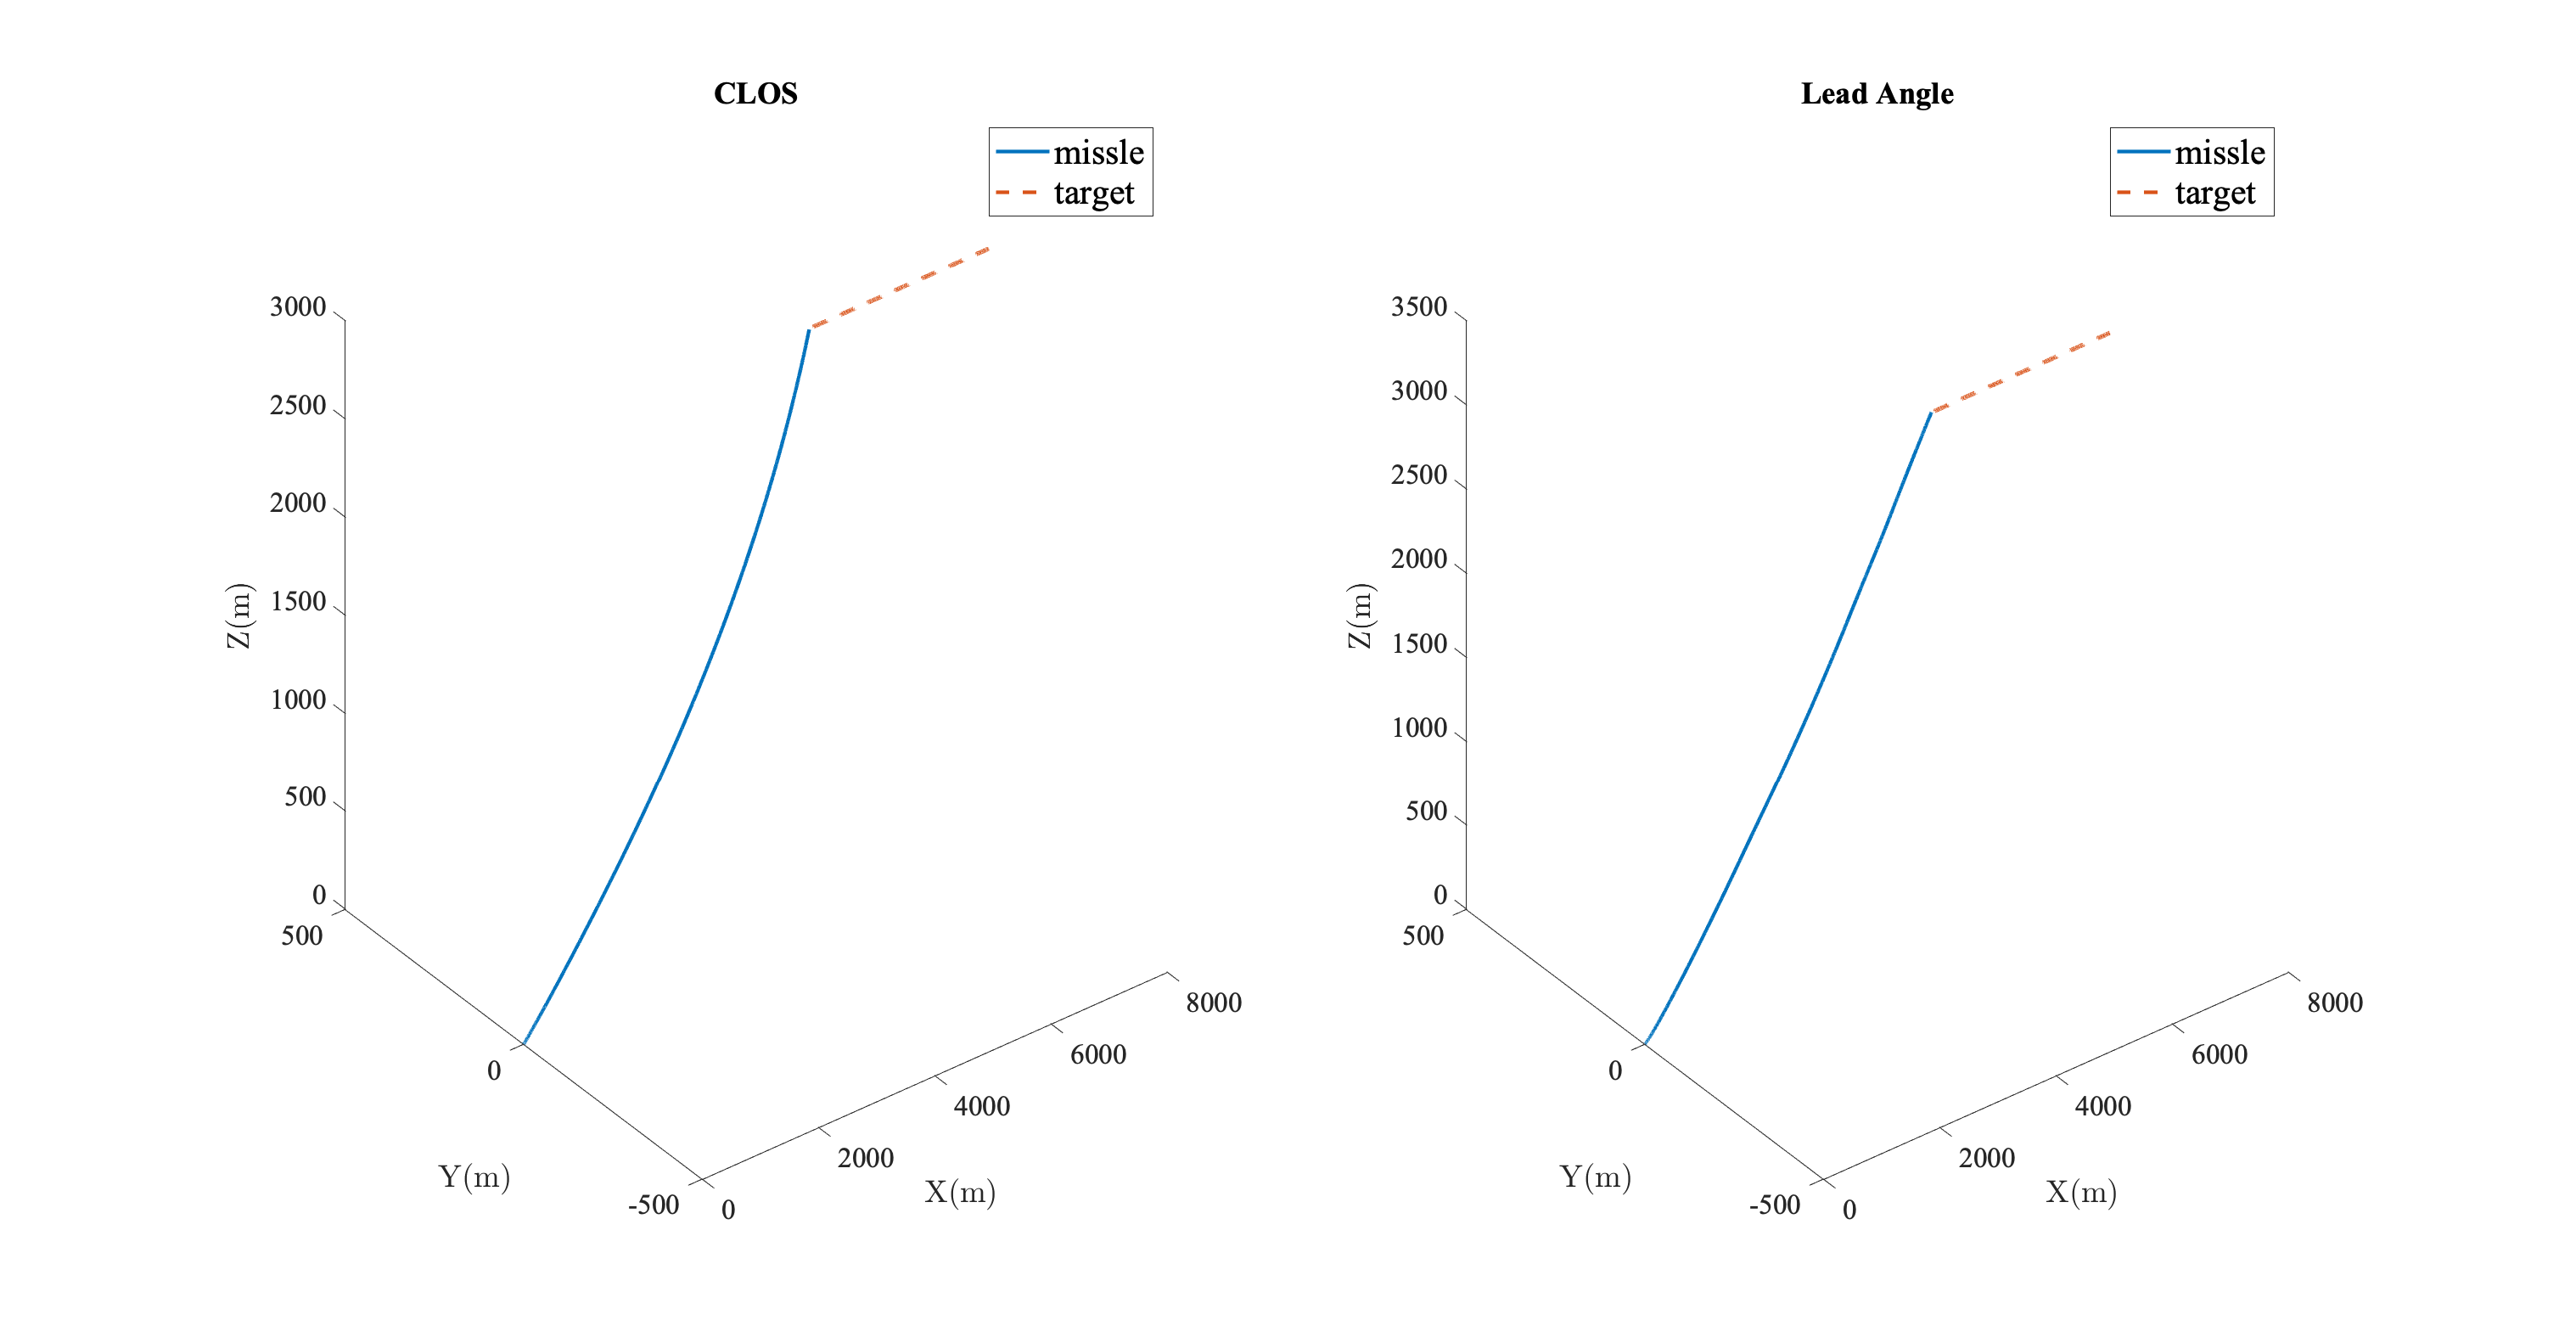
\includegraphics[width=\linewidth]{../Figure/j/3DoF_missle_vs_target_state_CLOS}
	\caption{مقایسه موقعیت موشک و هدف به صورت سه بعدی در دو نمودار  برای بررسی درنظرگرفتن زاویه پیشبین در قانون هدایت فرمان به خط دید}
\end{figure}


\begin{figure}[H]
	\centering
	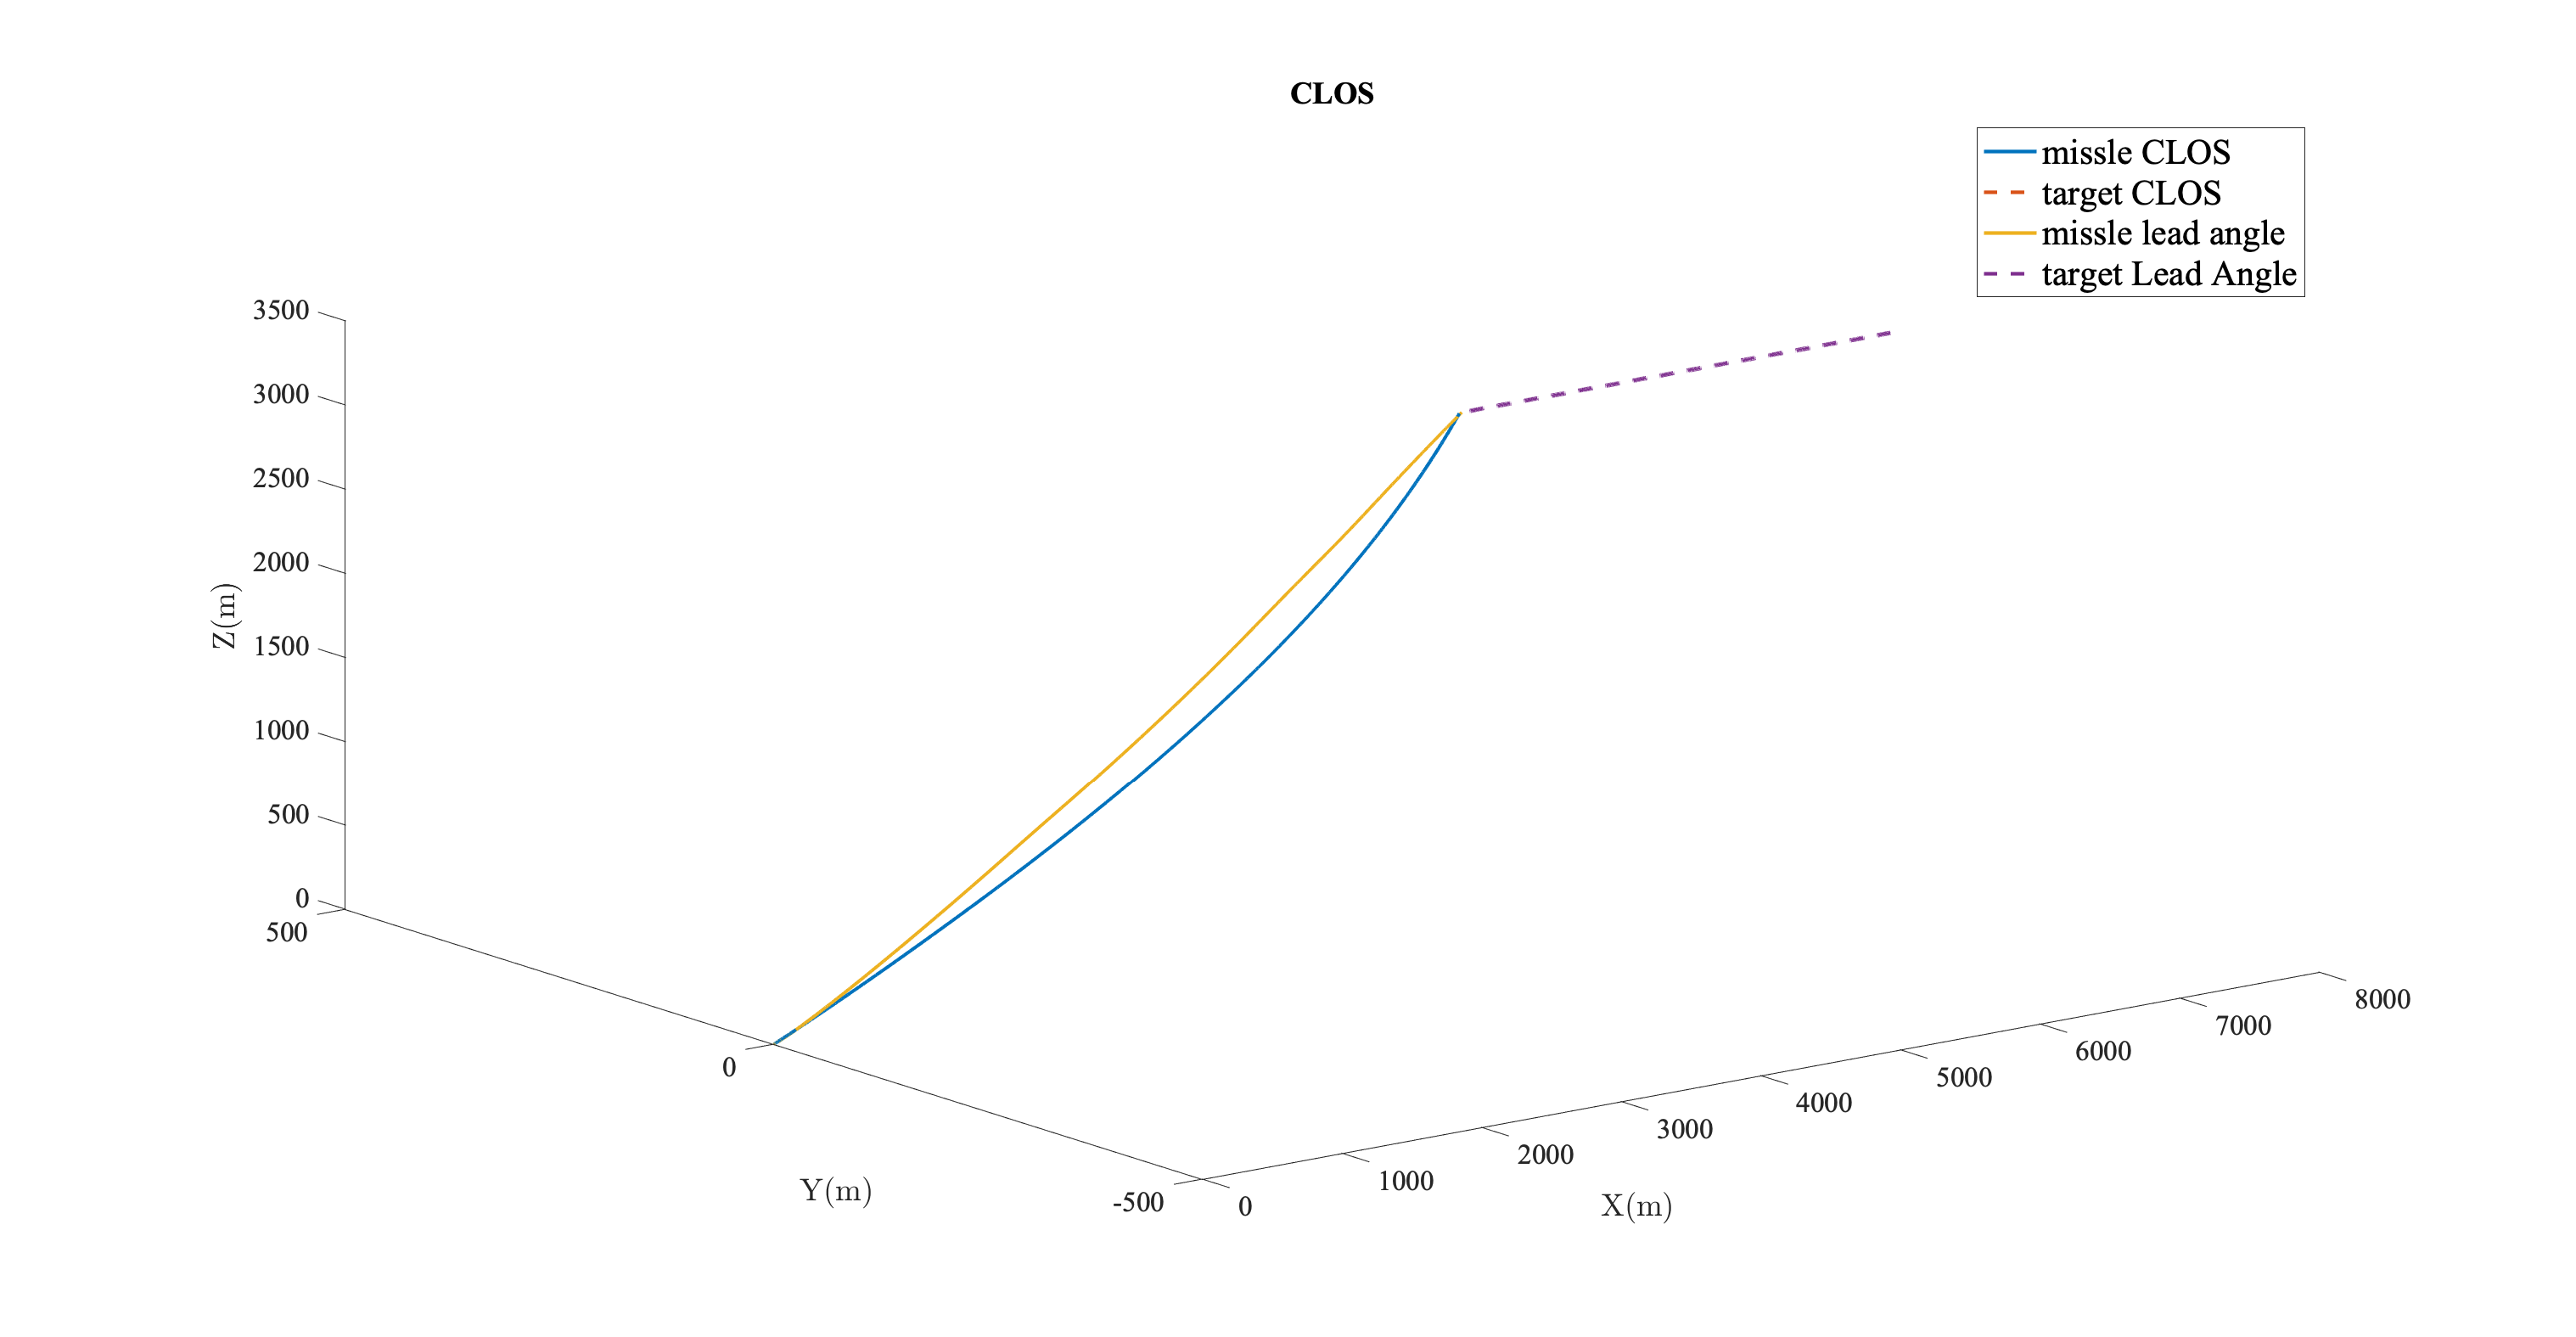
\includegraphics[width=\linewidth]{../Figure/j/3DoF_missle_vs_target_state_CLOS_all_in}
	\caption{مقایسه موقعیت موشک و هدف به صورت سه بعدی در یک نمودار برای بررسی درنظرگرفتن زاویه پیشبین در قانون هدایت فرمان به خط دید}
\end{figure}

\begin{figure}[H]
	\centering
	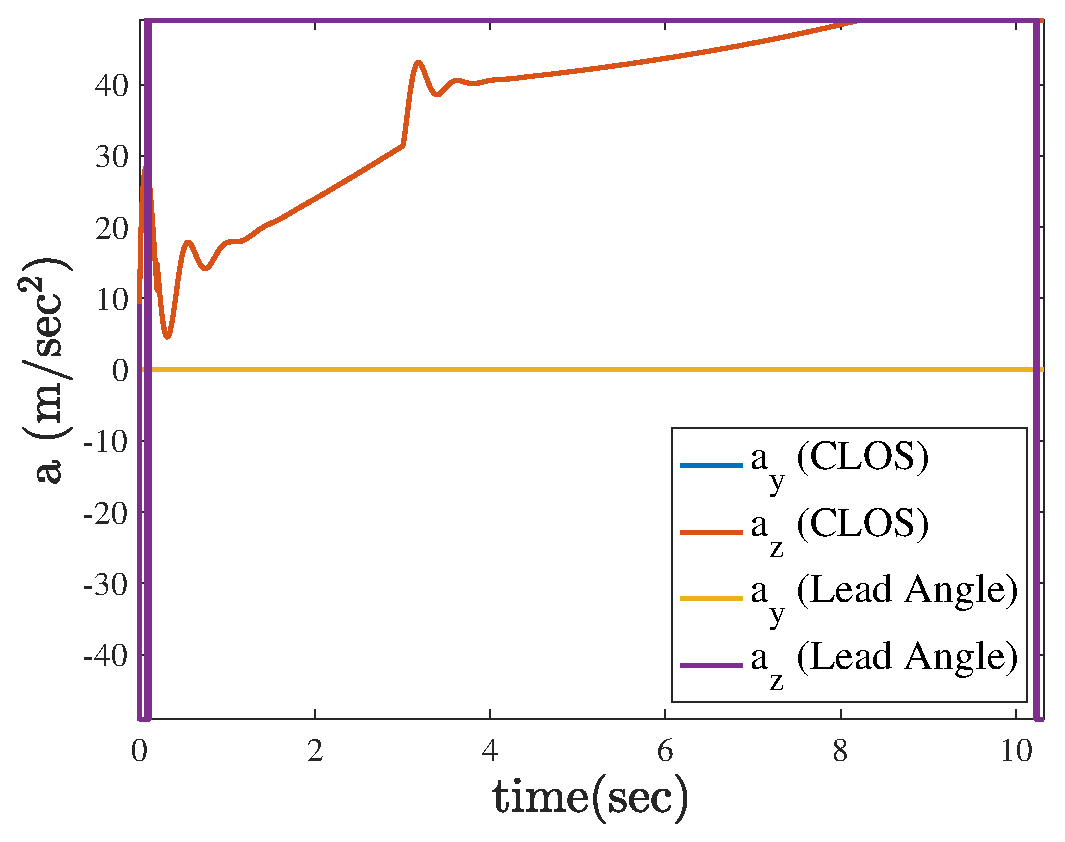
\includegraphics[width=.75\linewidth]{../Figure/j/command}
	\caption{مقایسه فرمان موشک برای بررسی درنظرگرفتن زاویه پیشبین در قانون هدایت فرمان به خط دید}
	
\end{figure}

\begin{figure}[H]
	\centering
	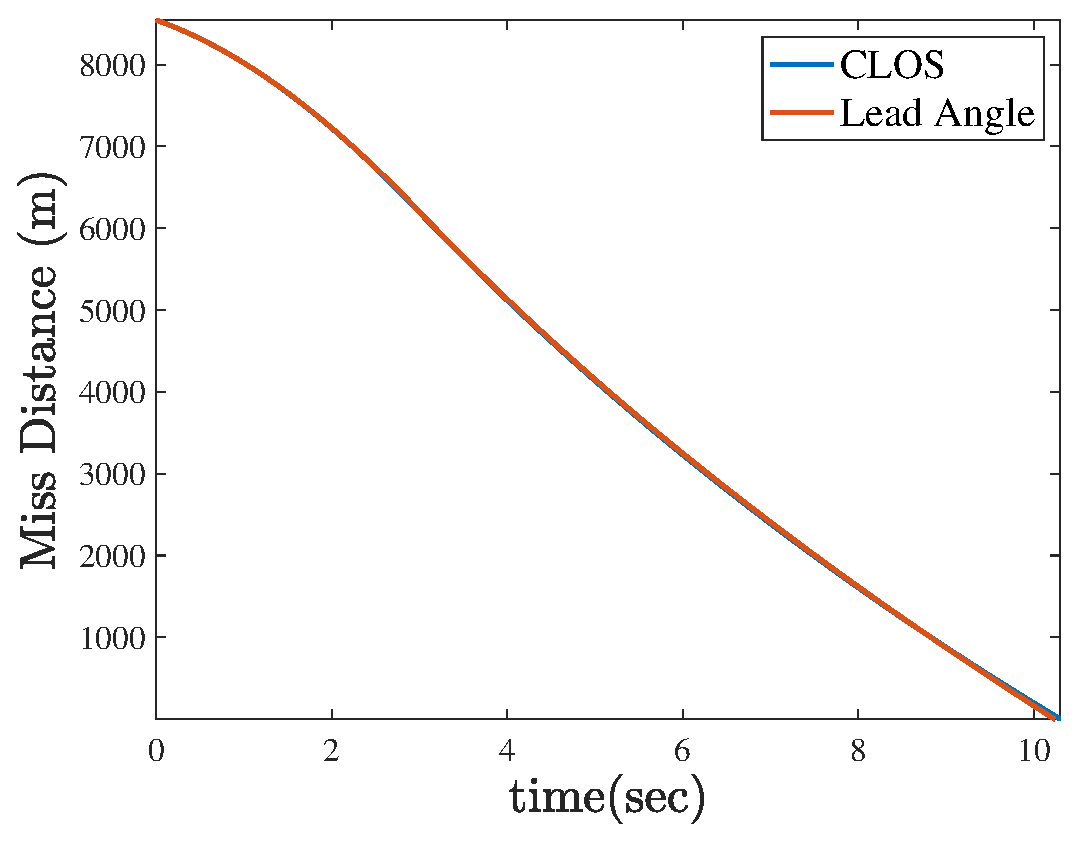
\includegraphics[width=.75\linewidth]{../Figure/j/miss_distance}
	\caption{مقایسه فاصله ازدست‌دهی موشک برای بررسی درنظرگرفتن زاویه پیشبین در قانون هدایت فرمان به خط دید}
\end{figure}

